\chapter{Az FPGA NES tesztelése}

Az FPGA-s projektek tesztelésének általában három nagy fázisa van. Az első a fejlesztői környezet szimulációs rendszerében futtatott tesztek. A második ezt követően az éles hardverrel futtatott tesztek. A teszteket végeztével az eredmények kiértékelése a harmadik fázis. Ezeket a teszt folyamatokat fogom bemutatni a diplomaterv projektemen, ebben a fejezetben.

\section{Rendszer szimulációk}

A legtöbb esetben egy FPGA-s fejlesztések során a tesztelések két csoportra bonthatóak: a modul tesztekre és a teljes rendszer tesztelésére. A NES projekt esetén viszont olyan komplex változásokat és bemeneteket kellett volna időzítéspontosan megadni a különálló modul tesztekhez (teljes CPU ciklusok processzor oldali műveletei), hogy inkább közvetlenül a teljes rendszer tesztelését kezdtem el.

A rendszer teszteket az ISE-n belül található ISim szimulátorában végeztem. Ezzel képesek vagyunk szintetizálható hardverek működési szimulációjára és az implementálás utáni, úgynevezett post-implemented rendszerek szimulálására is. A szintetizálható rendszerek esetében Verilog test fixture készítésével tudjuk meghatározni a szimulált jeleinket és szimulációs órajeleinket. A NES tesztkörnyezetének írása során a VGA modult és a hozzá tartozó elemeket kivettem a rendszerből, mivel ez csak extra számítást vett volna el a szimulátortól, illetve a rendszer időzítéseinek szinkronizálását is nehezebbé tette volna (50 MHz és 250 MHz-es órajelek arányainak megtartása a rendszer órajellel).

Ahhoz, hogy a teljes NES hardveremet szimulálhassam, szimulálhatóvá kellett tennem a konzulensemtől kapott 6502-es processzor futtatható binárisát. Ezt a feladatot az UNISIM konzol alkalmazás segítségével tudtam megoldani. Ez az eszköz azt teszi lehetővé, hogy implementált modulokból post-implemented szimulációs fájlt készít. Majd ehhez egy általunk értelmezhető Verilog input és output portokkal ellátott modult illeszt, ezáltal képesek vagyunk a kapott szimulációs fájt beilleszteni egy Verilog test fixture-be. A program futtatásához \aref{fig:UNISIM}. ábrán látható beállításokat alkalmaztam.

\begin{figure}[H]
	\centering
	\includegraphics[width=120mm, keepaspectratio]{figures/UNISIM}
	\caption{Az UNISIM konzol alkalmazás beállításai} 
	\label{fig:UNISIM}
\end{figure}

A szimulációkhoz és későbbiekben a hardveres tesztekhez is szükségünk van arra, hogy a Karakter és Program ROM-jaink helyes adatokat tartalmazzanak. A NES játékkártyák tartalma általában egy .nes bináris fájlban áll rendelkezésre. Ez tartalmaz egy 16 bájtos fejlécet, majd a program ROM-ot, végül pedig a karakter ROM-ot. A fejléc írja le, hogy az adott játék ROM-jai mekkora területet foglalnak, illetve a játék kártya milyen mapper-t tartalmaz. A .nes fájlt egy program segítségével könnyen felbonthatjuk két bináris ROM területre, majd egy egyszerű shell script segítségével szöveges fájlba írhatjuk a kapott binárisaink tartalmát. Majd az így kapott szöveges fájlok tartalmát a \$readmemh parancs segítségével tudjuk a blokk RAM-okba tölteni. A szimulációk kezdetén a helyes működéséhez érdemes még az összes használt memória területet 0-val feltölteni. Ezeknek az inicializációknak egy részét \aref{code:filling-RAM}. hardverleírásban olvashatjuk.

\begin{lstlisting}[caption={A memória területek inicializálása a szimulációs és hardveres tesztekhez}, label={code:filling-RAM}, style=prettyverilog]
//Character ROM initialization 
initial begin
	$readmemh( "src/games/DK_chr_rom_hex.txt" , ch_rom); //Super_Mario_Bros_chr_rom.txt
end

//NT RAM initialization 
reg  [7:0] 		name_table_ram [2047:0];
integer x;
initial begin for (x=0; x<2048; x=x+1) name_table_ram[x] = 8'b0;
end\end{lstlisting}

Azt tapasztaltam, hogy nagyobb és összetettebb rendszerek szimulációja során az ISim, hosszabb időtartalmú szimulációkra nem alkalmas (nem konzisztensek a számításai). Ezáltal csak egy adott pontig tudtam a szimulációkra hagyatkozni, viszont ez pont elégnek volt ahhoz, hogy könnyen elkezdhessem a teljes rendszer hardveres tesztelését.  

\newpage
\section{Hardveres tesztek}

A diplomatervem során sikerült elkészíteni a konzulensem segítségével az első verzióját az FPGA NES kártyának. Ez \aref{fig:PCB-Assembled}. ábrán látható. \Aref{sec:fpga-nes-board-summary}. fejezet során viszont már egy javított második verziót mutattam be (ezért láthatunk némi különbséget a két kártya elrendezése között). A második verzióra javítottam a flash chip FPGA-ba huzalozásán és két extra hangerő szabályzó gombot adtam a nyákhoz.

\begin{figure}[H]
	\centering
	\includegraphics[width=99mm, keepaspectratio, angle=90]{figures/nes-pcb-assembled-top}
	\includegraphics[width=99mm, keepaspectratio, angle=90]{figures/nes-pcb-assembled-botom}
	\caption{A kész FPGA NES kártya} 
	\label{fig:PCB-Assembled}
\end{figure}

A hardveres tesztelés során, a hardver binárisának feltöltésére a MIT-en fejlesztett, Logsys flash programozót használtam, ennek implementálását már a fentebbiekben olvashattuk (\ref{sec:logsysport}. fejezet). Az FPGA NES kártya mérési és tesztelési elrendezését \aref{fig:pcb-testing}. ábrán láthatjuk. 

A NES rendszer tesztelésére két klasszikus játékot választottam. Az első a Donkey Kong, amely egy könnyebben emulálható 16 kilobájtos program ROM-al rendelkező játék. A második pedig a NES egyik legnehezebben emulálható játéka, a Super Mario Bros. Ehhez a játékhoz hibátlanul implementált időzítésekre és helyesen kialakított PPU és CPU memória címekre van szükség. Ezt a játékot szokták legtöbbször a végső tesztként használni emulált PPU-k és CPU-k tesztelésére. A Donkey Kong tesztelését és futását \aref{fig:Donkey-start}. és \ref{fig:Donkey-level-1}. ábrákon láthatjuk. A Super Mario Bros.-t pedig futás közben \aref{fig:Super-Mario-start}. és \ref{fig:Super-Mario-world5-1}. ábrán tekinthetjük meg.
	
\begin{figure}[H]
	\centering
	\includegraphics[width=112mm, keepaspectratio, angle=90]{figures/nes-pcb-testing}
	\caption{FPGA NES kártya mérési és tesztelési elrendezésé} 
	\label{fig:pcb-testing}
\end{figure}

\begin{figure}[H]
	\centering
	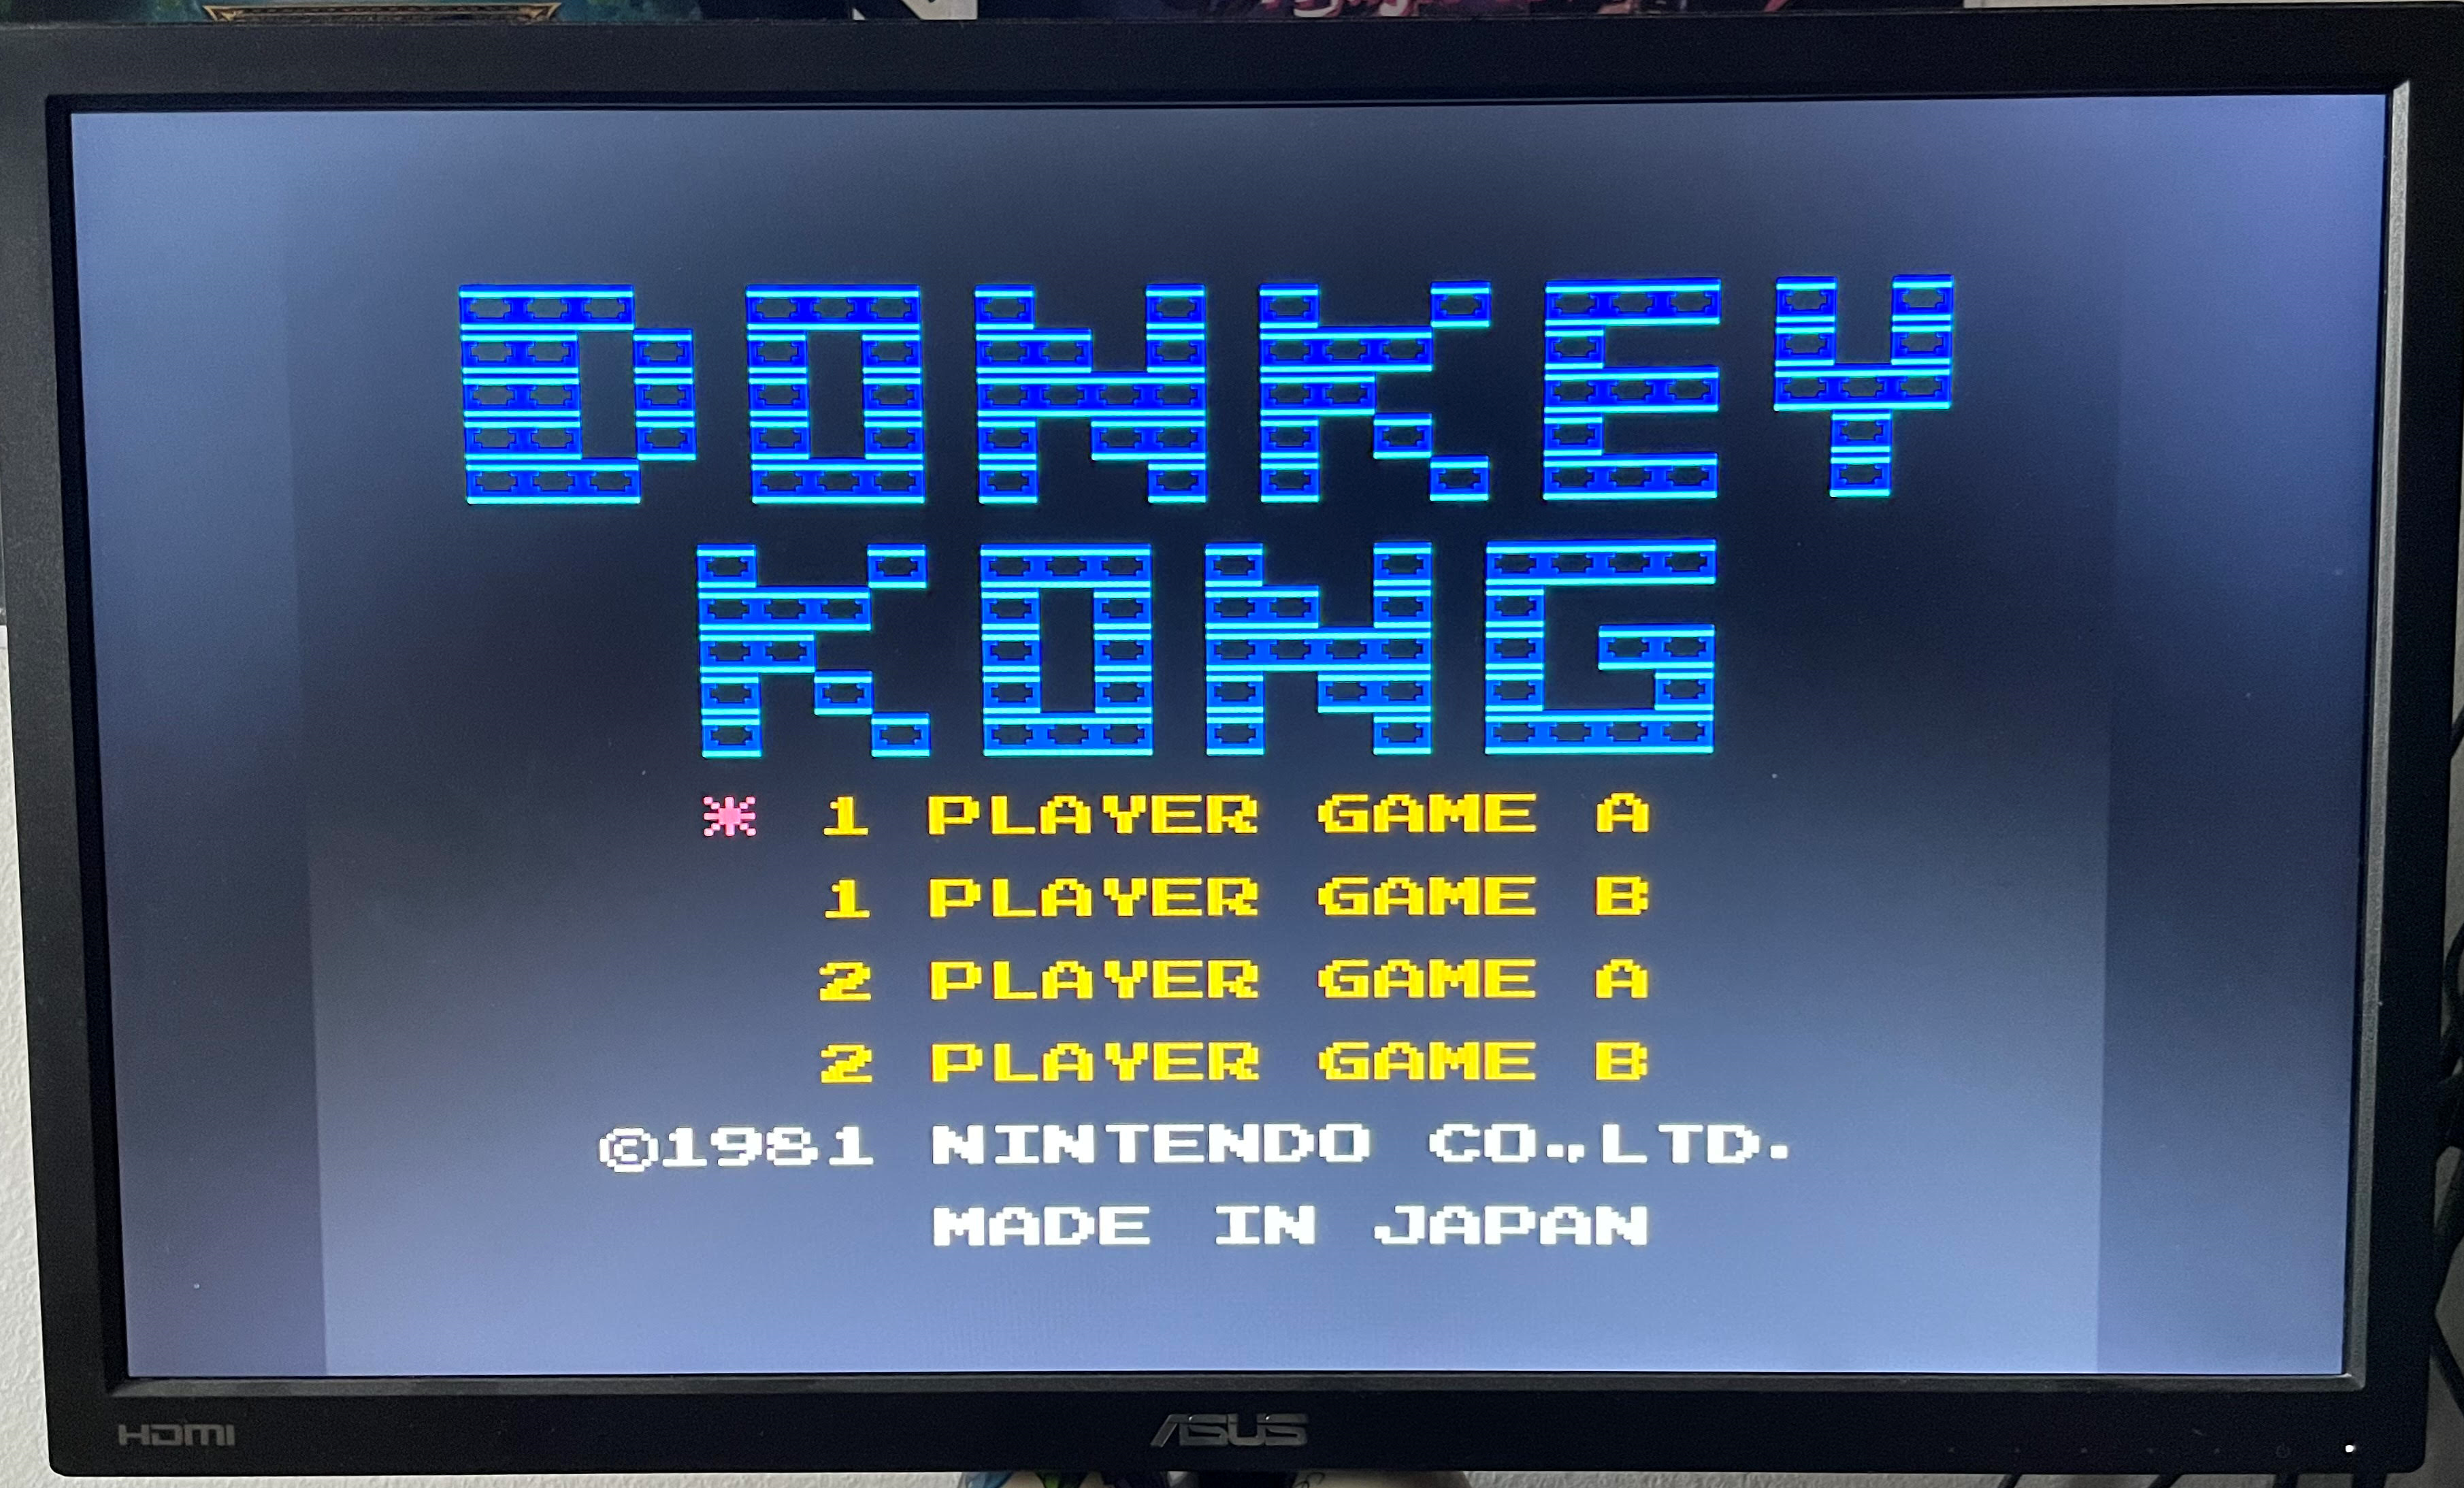
\includegraphics[width=150mm, keepaspectratio]{figures/Donkey-start}
	\caption{A Donkey Kong kezdő képernyője} 
	\label{fig:Donkey-start}
\end{figure}

\begin{figure}[H]
	\centering
	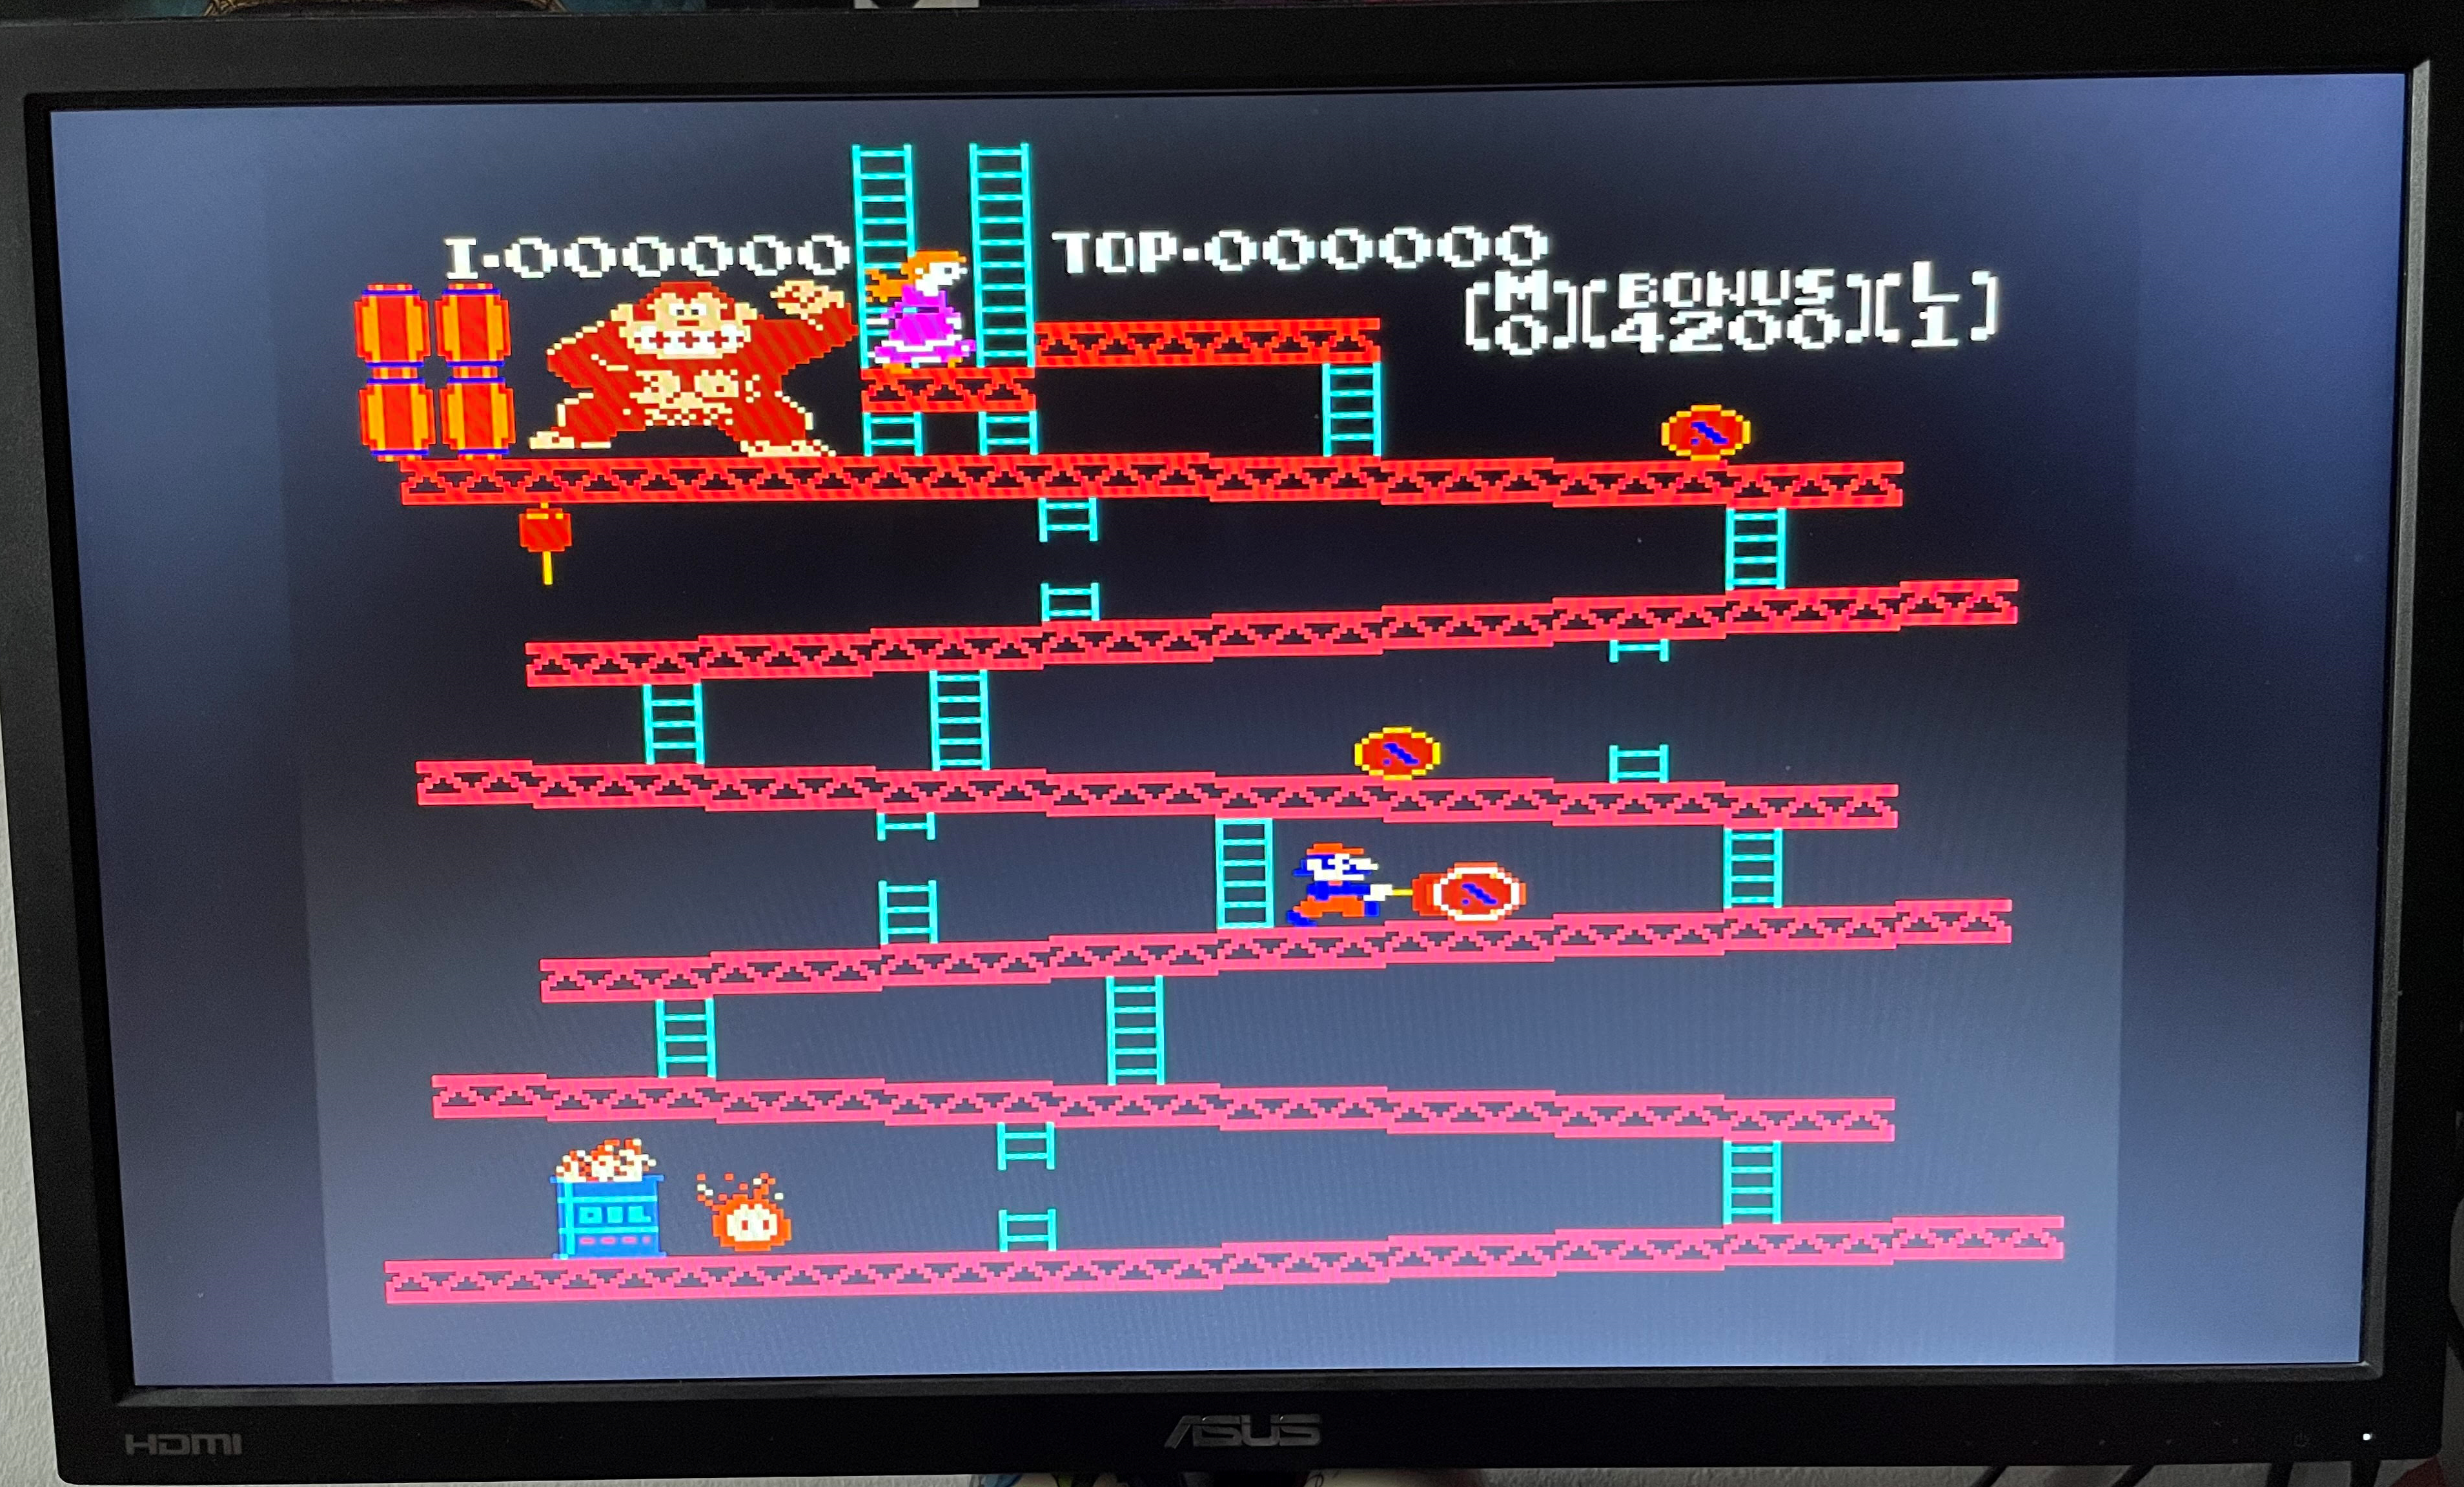
\includegraphics[width=150mm, keepaspectratio]{figures/Donkey-level-1}
	\caption{Donkey Kong ikonikus első pálya futás közben} 
	\label{fig:Donkey-level-1}
\end{figure}

\begin{figure}[H]
	\centering
	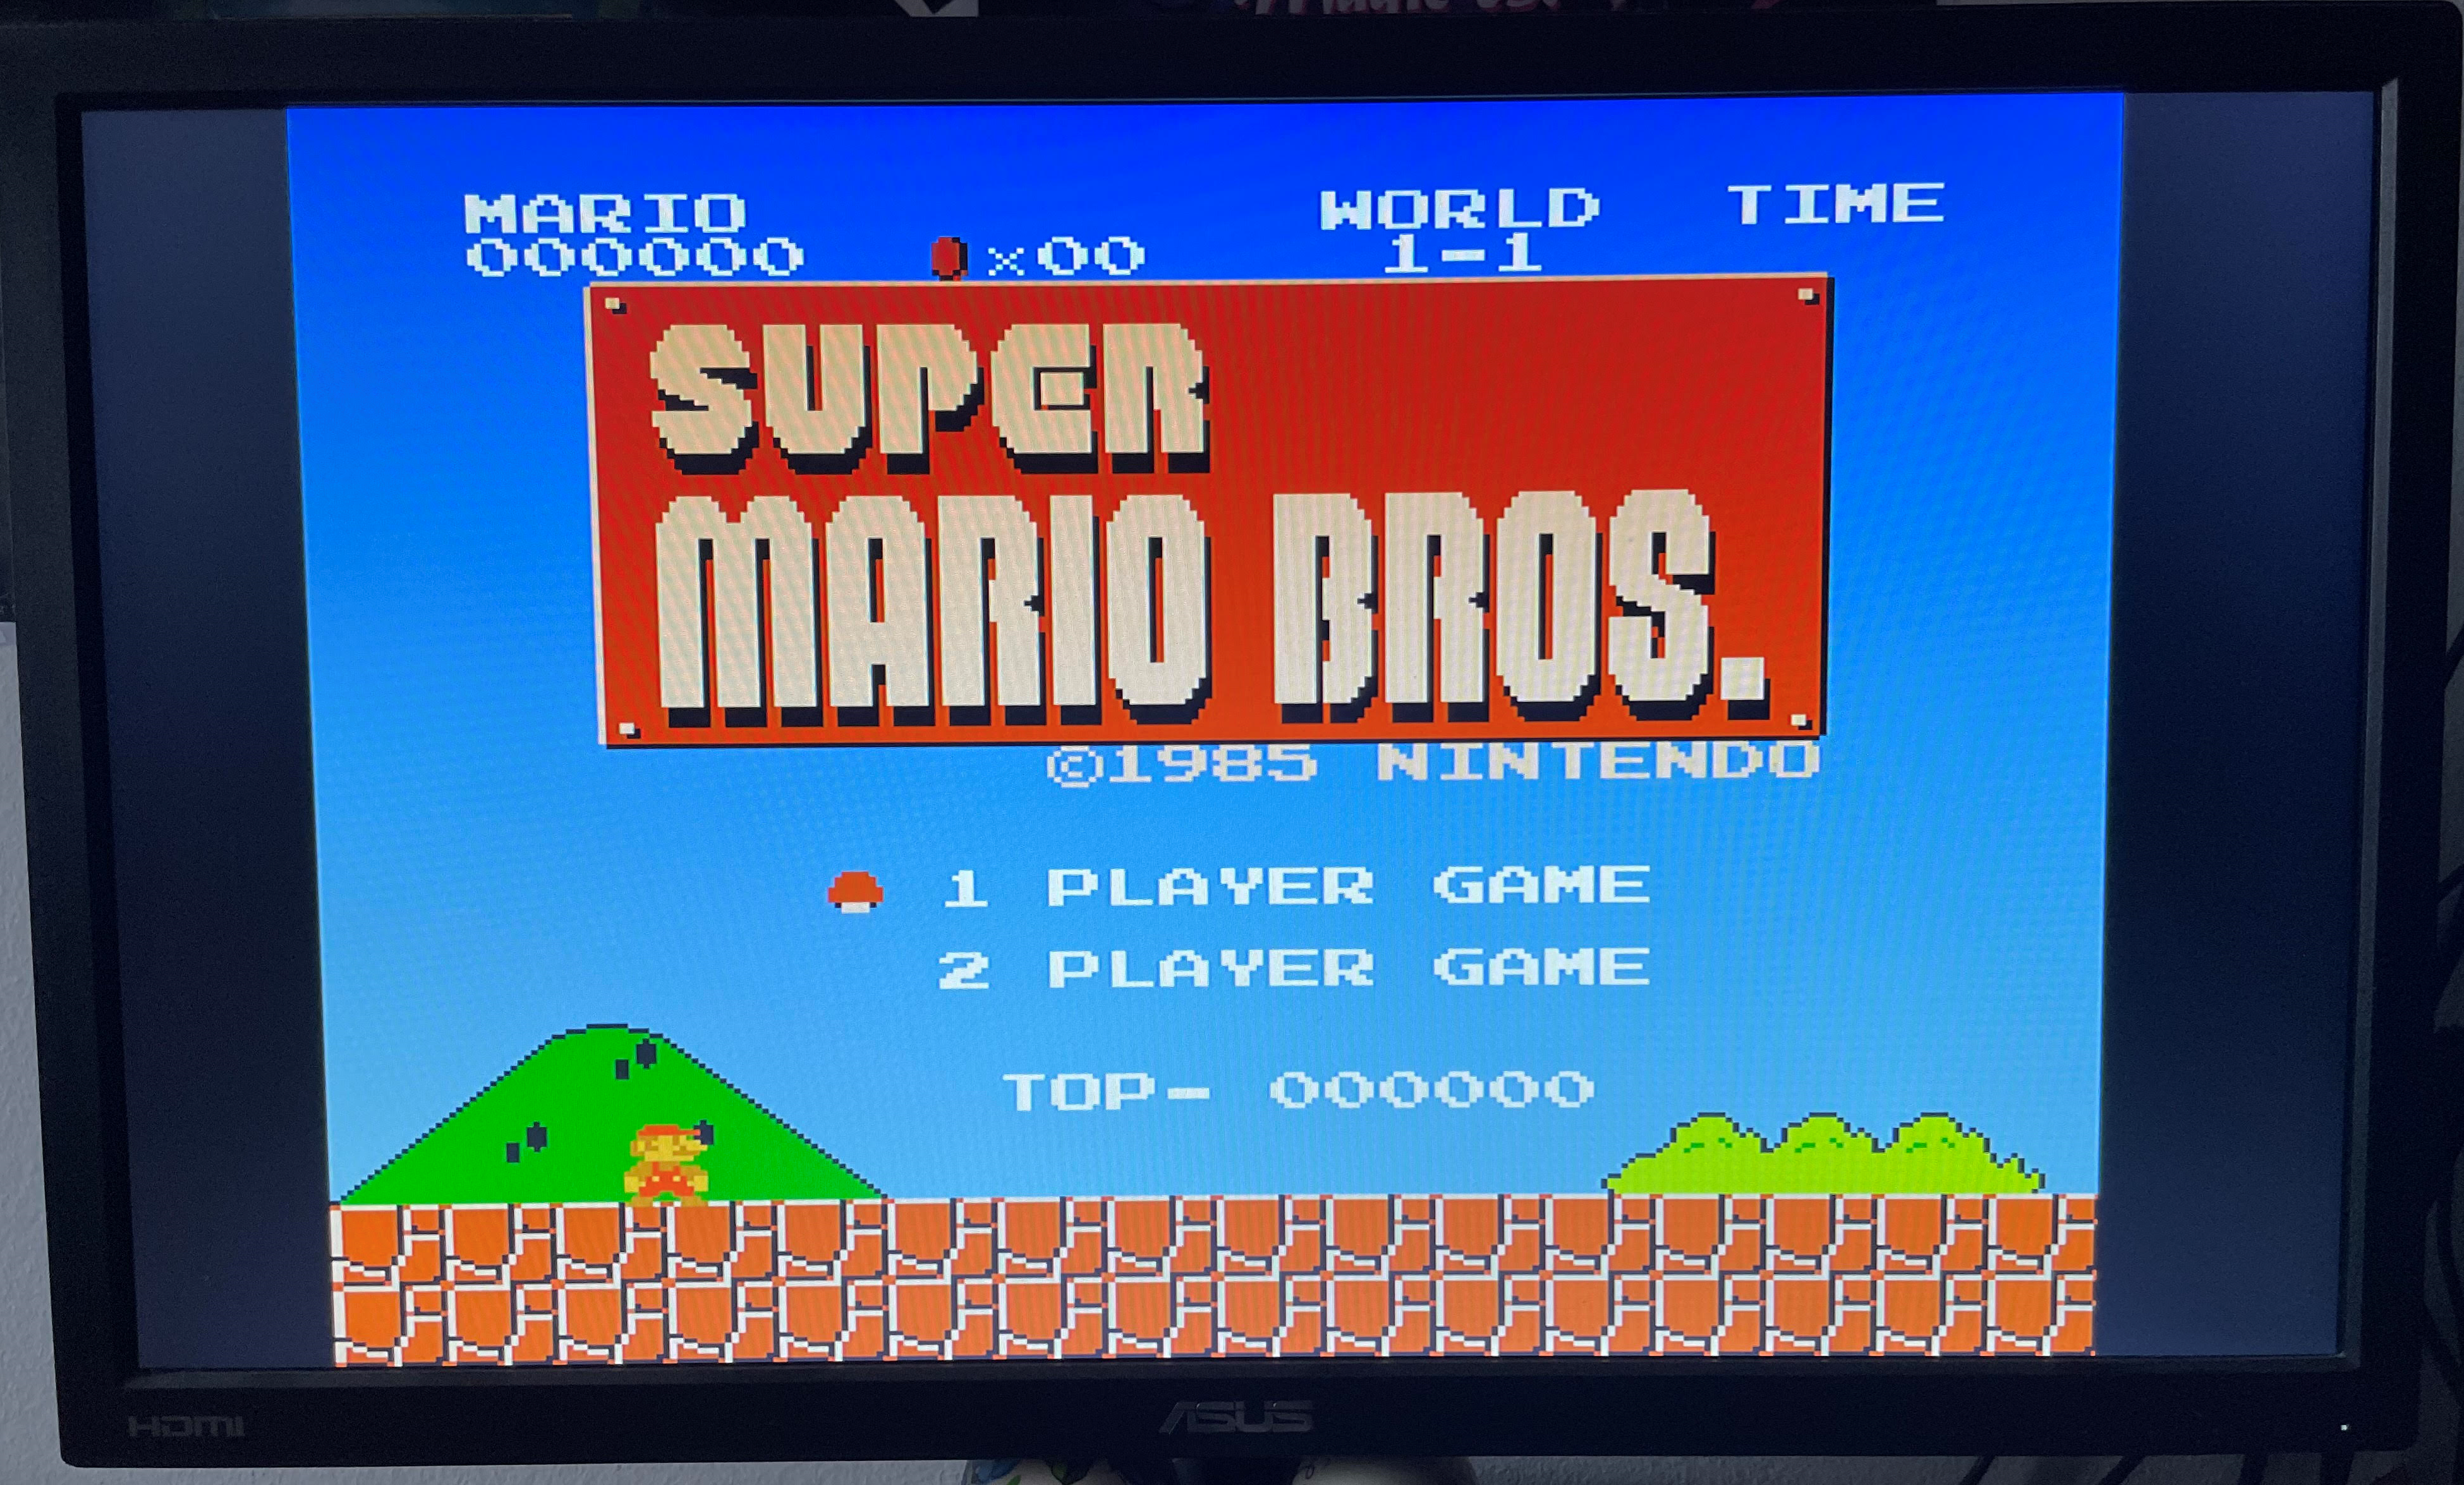
\includegraphics[width=150mm, keepaspectratio]{figures/Super-Mario_Start-croped}
	\caption{A Super Mario Bros. kezdő képernyője} 
	\label{fig:Super-Mario-start}
\end{figure}

\begin{figure}[H]
	\centering
	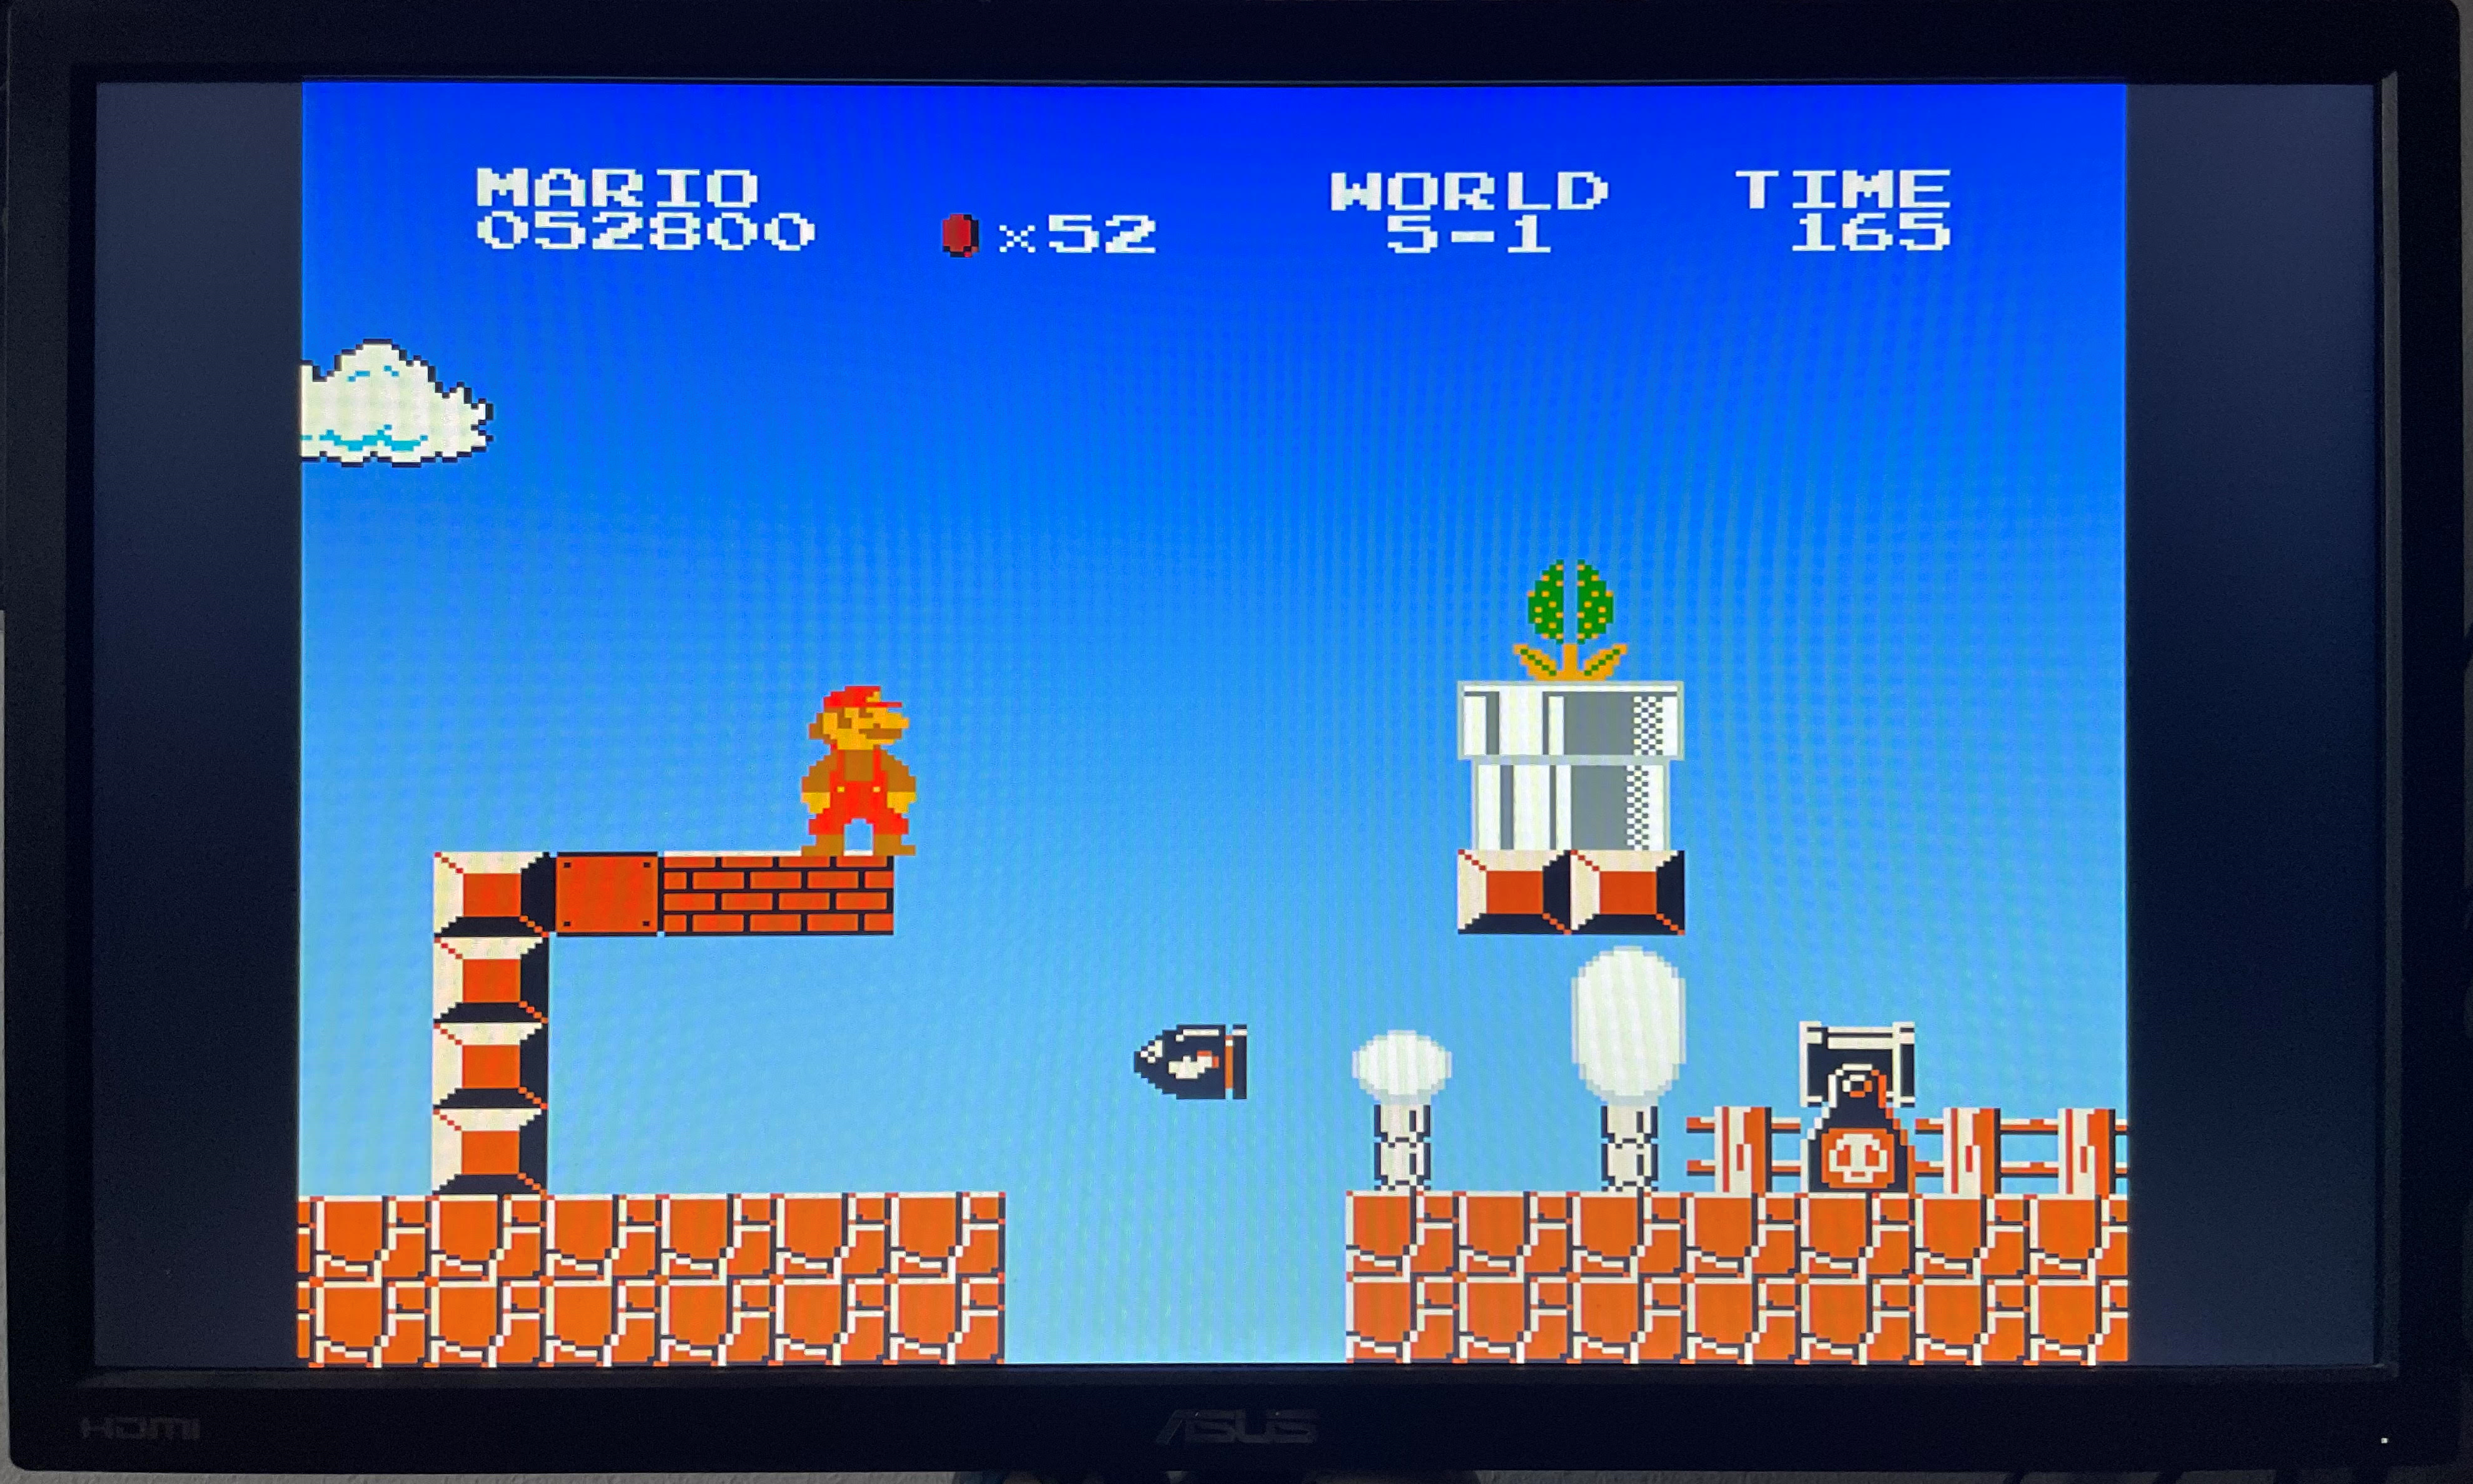
\includegraphics[width=150mm, keepaspectratio]{figures/Super-Mario-world5-1-croped}
	\caption{A Super Mario Bros. ötödik világának első pályája} 
	\label{fig:Super-Mario-world5-1}
\end{figure}

\section{A tesztek eredményeinek kiértékelése}

A szimulációs tesztek során sikeresen fel tudtam éleszteni a NES rendszerét olyan szintre, hogy elkezdhettem a hardveres teszteket. A későbbiek során is voltak olyan hardveres modulok, amelyekben hibakeresés során többször is visszanyúltam a szimulátorhoz. Sajnos a ISim hibás működése miatt a teljes rendszert nem tudtam nyomon követni, viszont a szimulációk során megfigyelt hardveres működéseket \aref{sec:fpga-desing-begining}. fejezetben több helyen is láthatjuk.

A hardveres tesztelések eredménye is sikeres lett, a két játék teljes mértékben játszható állapotban van. A hosszabb tesztelések során sem akadtam olyan hibára, amely a programok futását megakadályoznák és ezzel a játékokat játszhatatlanná tennék. A képalkotásért felelős chip a PPU időzítései is pontosak, hiszen még az idő kritikus játékok, mint a Mario is játszható a konzolon. Ez \aref{fig:Super-Mario-world5-1}. ábrán is látható. Itt még jól megfigyelhető az is, hogy a PPU háttér és sprite alkotási része is összhangban van (egy sűrűbb mozgó elemekkel teli képen sem hibásodik meg a képalkotás). Az általam használt színpaletták, szépen visszaadják az eredeti NES játékok színvilágát, ezzel egy nagyon jó minőségű emulálást lehetővé téve.

Úgy érzem az FPGA-s hardverfejlesztések teszteléseinek széleskörű tárházát ismertem meg, és ezen eszközök segítségével sikeresen működésre bírtam az általam fejlesztett konzol hardverét.